\documentclass[10pt]{article}
\usepackage{fullpage}
\usepackage{amsmath}
\usepackage[amsthm, thmmarks]{ntheorem}
\usepackage{amssymb}
\usepackage{graphicx}
\usepackage{enumerate}
\usepackage{verse}
\usepackage{tikz}
\usepackage{verbatim}
\usepackage{hyperref}
\usepackage{algpseudocode}
\usepackage{algorithm}

\newtheorem{lemma}{Lemma}
\newtheorem{theorem}[lemma]{Theorem}
\newtheorem{definition}[lemma]{Definition}
\newtheorem{proposition}[lemma]{Proposition}
\newtheorem{corollary}[lemma]{Corollary}
\newtheorem{claim}[lemma]{Claim}
\newtheorem{example}[lemma]{Example}

\newcommand{\dee}{\mathrm{d}}
\newcommand{\Dee}{\mathrm{D}}
\newcommand{\In}{\mathrm{in}}
\newcommand{\Out}{\mathrm{out}}
\newcommand{\pdf}{\mathrm{pdf}}
\newcommand{\Cov}{\mathrm{Cov}}
\newcommand{\Var}{\mathrm{Var}}

\newcommand{\ve}[1]{\mathbf{#1}}
\newcommand{\ves}[1]{\boldsymbol{#1}}
\newcommand{\mrm}[1]{\mathrm{#1}}
\newcommand{\etal}{{et~al.}}
\newcommand{\sphere}{\mathbb{S}^2}
\newcommand{\modeint}{\mathcal{M}}
\newcommand{\azimint}{\mathcal{N}}
\newcommand{\ra}{\rightarrow}
\newcommand{\mcal}[1]{\mathcal{#1}}
\newcommand{\X}{\mathcal{X}}
\newcommand{\Y}{\mathcal{Y}}
\newcommand{\Z}{\mathcal{Z}}
\newcommand{\x}{\mathbf{x}}
\newcommand{\y}{\mathbf{y}}
\newcommand{\z}{\mathbf{z}}
\newcommand{\tr}{\mathrm{tr}}
\newcommand{\sgn}{\mathrm{sgn}}
\newcommand{\diag}{\mathrm{diag}}
\newcommand{\Real}{\mathbb{R}}
\newcommand{\sseq}{\subseteq}
\newcommand{\ov}[1]{\overline{#1}}
\newcommand{\data}{\mathrm{data}}

\DeclareMathOperator*{\argmax}{arg\,max}
\DeclareMathOperator*{\argmin}{arg\,min}


\title{Algorithms for Non-Linear Least Squares}
\author{Pramook Khungurn}

\begin{document}
\maketitle

This note is written as I study algorithms for the non-linear least squares problem, which will culminate in the Levenberg--Marquardt algorithm. Source materials I use for this note includes Madsen \etal~\cite{Madsen:2004}, Frandsen \etal~\cite{Frandsen:2004}, and Norcedal and Wright~\cite{Norcedal:2006}.

\section{Notations}

\begin{itemize}
    \item Scalars are denoted by regular (i.e., non-bold, non-italic) small latters: $a$, $b$, $c$, $x$, $y$, and $z$.
    \item We denote vectors with bold, small letters: $\ve{a}$, $\ve{b}$ $\ve{c}$, $\ve{x}$, $\ve{y}$, and $\ve{z}$.
    \item Vector components are denoted with regular, small letters with a subscript. For example, $$\ve{x} = (x_1, x_2, \dots, x_n).$$
    \item Matrices, on the other hand, are denoted by regular, capital letters: $A$, $B$, and $C$.
    \item Scalar functions use the same type face as scalars, and vector functions use the same type face as vectors.
    \item Component functions of vector functions are denoted in the same was a vector components. That is, if $f: \Real^n \ra \Real^m$, then
    \begin{align*}
        \ve{f}(\ve{x}) = \begin{bmatrix} f_1(\ve{x}) \\ f_2(\ve{x}) \\ \vdots \\ f_m(\ve{x}) \end{bmatrix}.
    \end{align*}
    \item For derivatives, we use the notations I developed in a previous note \cite{Khungurn:2022}.
\end{itemize}

\section{Preliminary}

\begin{itemize}
    \item We are interested in solving the {\bf non-linear least squares} problem. That is, we are given a non-linear vector function $\ve{f}: \Real^n \ra \Real^m$, and we want to find $\ve{x}^*$ such that $\| \ve{f}(\ve{x}^*) \|^2$ is minimized. In other words, we want to compute
    \begin{align*}
        \ve{x}^* = \argmin_{\ve{x}} \big\{ \| \ve{f}(\ve{x}) \|^2 \big\}.
    \end{align*}

    \item Of course, non-linear least square is a special case of the general {\bf function minimization} problem. Here, we are given a {\bf loss function}, aka an {\bf objective function}, $\mcal{L}: \Real^n \ra \Real$. We want to find
    \begin{align*}
        \ve{x}^* = \argmin_{\ve{x}} \big\{ \mcal{L}(\ve{x}) \big\}.
    \end{align*}

    \item Obviously, for the non-linear least square problem, we have that $\mcal{L}(\ve{x}) = \| \ve{f}(\ve{x}) \|^2$.
    
    \item Finding $\argmin_{\ve{x}} \{ \mcal{L}(\ve{x}) \}$ (i.e., the {\bf global minimizer}) is very hard in general, especially with non-linear $\ve{f}$. So, we settle to find a local minimizer instead.
    
    \begin{definition}
        A point $\ve{x} \in \Real^n$ is said to be a {\bf local minimizer} of $\mcal{L}: \Real^n \ra \Real$ if there exists $\delta > 0$ such that $\mcal{L}(\ve{x}') \leq \mcal{L}(\ve{x})$ for all $\| \ve{x} - \ve{x}' \| < \delta$. In other words, there exists a neighborhood of $\ve{x}$ such that $\mcal{L}(\ve{x})$ is minimal.
    \end{definition}

    \item We shall assume that $\mcal{L}$ is differentiable to arbitrary order. As a result, we have that
    \begin{align*}
        \mcal{L}(\ve{x} + \ve{h}) = \mcal{L}(\ve{x}) + \nabla\mcal{L}(\ve{x}) \ve{h} + \frac{1}{2} \ve{h}^T H_{\mcal{L}}(\ve{x}) \ve{h} + O(\| \ve{h} \|^3)
    \end{align*}
    where $H_{\mcal{L}}(\ve{x})$ denotes the Hessian matrix of $\mcal{L}$:
    \begin{align*}
        H_{\mcal{L}}(\ve{x}) = \begin{bmatrix}
            \nabla_{1,1} \mcal{L}(\ve{x}) & \nabla_{1,2} \mcal{L}(\ve{x}) & \cdots & \nabla_{1,n} \mcal{L}(\ve{x}) \\
            \nabla_{2,1} \mcal{L}(\ve{x}) & \nabla_{2,2} \mcal{L}(\ve{x}) & \cdots & \nabla_{2,n} \mcal{L}(\ve{x}) \\
            \vdots & \vdots & \ddots & \vdots \\
            \nabla_{n,1} \mcal{L}(\ve{x}) & \nabla_{n,2} \mcal{L}(\ve{x}) & \cdots & \nabla_{n,n} \mcal{L}(\ve{x})           
        \end{bmatrix}
        = \nabla((\nabla \mcal{L}(\ve{x}))^T).
    \end{align*}

    \item \begin{definition}
        A point $\ve{x} \in \Real^n$ is said to be a {\bf stationary point} of $\mcal{L}: \Real^n \ra \Real$ if $\nabla{L}(\ve{x}) = \ve{0}^T$.
    \end{definition}

    \item \begin{theorem}
        A local minimizer of $\mcal{L}$ is a stationary point.
    \end{theorem}
    In other words, being a staionary point is a necessary condition for being a local minimizer. It is not a sufficient condition because a stationary point can be a \emph{local maximizer} or a \emph{saddle point}      

    \item The sufficient condition for a local minimizer is given below.
    \begin{theorem}
        If $\ve{x}$ is a stationary point of $\mcal{L}$, and $H_{\mcal{L}}(\ve{x})$ is positive definite, then $\ve{x}$ is a local minimizer.
    \end{theorem}
\end{itemize}

\section{Descent Methods}

\begin{itemize}
    \item In this section, we present methods for the general function minimzation problem. We will deal with methods specific to non-linear least squares in the sections after this one.
    
    \item The methods in this section are iterative.
    \begin{itemize}
        \item Start with a starting point $\ve{x}^{(0)}$.
        \item We produce a series of points $\ve{x}^{(1)}$, $\ve{x}^{(2)}$, $\dotsc$.
    \end{itemize}
    Then, we pray that the series of points would converge to a local minimizer $\ve{x}^*$.

    \item Let $\ve{e}^{(k)} = \ve{x}^{(k)} - \ve{x}^*.$ The optimization process converges if $\lim_{k \ra \infty} \| \ve{e}^{(k)}\| = 0$.
    
    \item We are interested in quantifying how the optimization process converges. The speed at which it converges can be measured by how much $\| \ve{e}^{(k+1)} \|$ becomes smaller than $\| \ve{e}^{(k)} \|$. There are multiple types of convergence
    \begin{itemize}
        \item {\bf Linear convergence} is when $\| \ve{e}^{(k+1)}\| \leq a\| \ve{e}^{(k)} \|$ for some $0 < a < 1$ for all $k$ large enough.
        \item {\bf Quadratic convergence} is when $\| \ve{e}^{(k+1)}\| = O(\| \ve{e}^{(k)} \|^2)$ for all $k$ large enough that $\| \ve{e}^{(k)} \|$ is small.
        \item {\bf Superlinear convergence} is when $\| \ve{e}^{(k+1)}\| / \| \ve{e}^{(k)}\| \ra 0$ as $k \ra \infty$.
    \end{itemize}

    \item Most methods try to ensure the \emph{descending condition}
    \begin{align*}
        \mcal{L}(\ve{x}^{(k+1)}) < \mcal{L}(\ve{x}^{(k)})
    \end{align*}
    for all $k \geq 0$. This prevents convergence to a local maximizer. However, we might still end up at a saddle point, but it is quite unlikely because a saddle point has directions that would increase the loss function's value. A {\bf descent method} is one that tries to maintain the descending condition.

    \item All methods in this note is a descent method with a particular structure. In each iteration of such a method, we do the following.
    \begin{itemize}
        \item Find a direction $\ve{h}$ along which to move $\ve{x}^{(k)}$. (Here, $k$ is the index of the iteration.)
        \item Find the step length to move $\ve{x}^{(k)}$.
    \end{itemize}
    
    \item The outline of the descent method is given in Algorithm~\ref{algo:descent-method}.
    
    \begin{algorithm}[t]
    \begin{algorithmic}
        \State $\ve{x} \gets \ve{x}^{(0)}$
        \While {{\bf true}}
            \State $\ve{h} \gets \Call{Find-Direction}{\ve{x}}$
            \If {(no such $\ve{h}$ exists)}
                \State \Return $\alpha$
            \Else
                \State $\alpha \gets \Call{Compute-Step-Length}{\ve{x}, \ve{h}}$
                \State $\ve{x} \gets \ve{x} + \alpha\ve{h}$            
            \EndIf
        \EndWhile
    \end{algorithmic}
    \caption{Descent method}
    \label{algo:descent-method}
    \end{algorithm}

    \item Consider how the value of $\mcal{L}$ changes after the update.
    \begin{align*}
        \mcal{L}(\ve{x} + \alpha \ve{h}) 
        &= \mcal{L}(\ve{x}) + \alpha \nabla \mcal{L}(\ve{x}) \ve{h} + O(\alpha^2) 
        \approx \mcal{L}(\ve{x}) + \alpha \nabla \mcal{L}(\ve{x}) \ve{h}
    \end{align*}
    when $\alpha$ is small enough. 
    
    \item \begin{definition}
        A direction $\ve{h}$ is a {\bf descent direction} if $\nabla \mcal{L}(\ve{x}) \ve{h} < 0$.
    \end{definition}

    \item If we are at $\ve{x}$ where there exists no descent direction, it must be that $\nabla \mcal{L}(\ve{x}) = \ve{0}$, so $\ve{x}$ is a stationary point.
    
    \item If there is a descent direction, we then have to find the step length $\alpha$ such that $\mcal{L}(\ve{x} + \alpha \ve{h}) < \mcal{L}(\ve{x}).$ 
\end{itemize}

\subsection{Gradient Descent}

\begin{itemize}
    \item One of the most popular descent method is {\bf gradient descent}. It chooses $\ve{h} = -(\nabla \mcal{L}(\ve{x}))^T$  and $\alpha$ to be a fixed small constant.
    
    \item The choice of the descent direction is the best choice locally at $\ve{x}^{(k)}$.
    
    \item However, the convergence of gradient descent is linear and often very slow.
    
    \item Nevertheless, it offers good performance when $\ve{x}$ is far away the converged solution $\ve{x}^*$. So, it is often used as the initial phase of the iterative optimization process.
\end{itemize}

\subsection{Newton's Method}

\begin{itemize}
    \item If $\ve{x}^*$ is a stationary point then, $\nabla \mcal{L}(\ve{x}^*) = \ve{0}$.
    
    \item We also have that
    \begin{align*}
        \nabla \mcal{L}(\ve{x} + \ve{h})^T
        &= \nabla \mcal{L}(\ve{x})^T + \nabla(\nabla \mcal{L}(\ve{x})^T) \ve{h} + O(\| \ve{h} \|^2) \\
        &= \nabla \mcal{L}(\ve{x})^T + H_{\mcal{L}}(\ve{x}) \ve{h} + O(\| \ve{h} \|^2) \\
        &\approx \nabla \mcal{L}(\ve{x})^T + H_{\mcal{L}}(\ve{x}) \ve{h}
    \end{align*}
    when $\| \ve{h} \|$ is small enough.

    \item Assuming that we can get to the stationary point in one step, it must be the case that $\nabla \mcal{L}(\ve{x} + \ve{h})^T = \ve{0}$. So,
    \begin{align*}
        \ve{0} &\approx \nabla \mcal{L}(\ve{x})^T + H_{\mcal{L}}(\ve{x}) \ve{h}.
    \end{align*}
    We go one step further and assume that the above inequality is an equality.
    \begin{align*}
        \ve{0} &= \nabla\mcal{L}(\ve{x})^T + H_{\mcal{L}}(\ve{x}) \ve{h}.
    \end{align*}
    This gives
    \begin{align*}
        \ve{h} = - (H_{\mcal{L}}(\ve{x}))^{-1} \nabla\mcal{L}(\ve{x})^T.
    \end{align*}

    \item {\bf Newton's method} chooses $\ve{h} = - (H_{\mcal{L}}(\ve{x}))^{-1} \nabla\mcal{L}(\ve{x})^T$ and $\alpha = 1$.
    
    \item If $H_{\mcal{L}}(\ve{x})$ is positive definite, we have that
    \begin{align*}
        0 < \ve{h}^T H_{\mcal{L}}(\ve{x}) \ve{h}.
    \end{align*}
    Because of our choice of $\ve{h}$, we have that $H_{\mcal{L}}(\ve{x}) \ve{h} = -\mcal{L}(\ve{x})^T$. As a result,
    \begin{align*}
        0 &< - \ve{h}^T \mcal{L}(\ve{x})^T \\
        \mcal{L}(\ve{x})^T \ve{h} &< 0.
    \end{align*}
    As a result, $\ve{h}$ is a descent direction if $H_{\mcal{L}}(\ve{x})$ is positive definite.

    \item Newton's method is good at a late stage of the optimization process. That is, whne $\ve{x}$ is close to $\ve{x}^*$. If $\ve{x}^*$ is a local minimizer, then $H_{\mcal{L}}(\ve{x}^*)$ is positive definite. As a result, there is a neighborhood around $\ve{x}^*$ such that, if $\ve{x}$ is in that neighborhood, then $H_{\mcal{L}}(\ve{x})$ is also positive definite. As a result, we have that $\ve{h}$ is a descent direction. Moreover, the convergence in this neighborhood is quadratic.
    
    \item On the other hand, if the $H_{\mcal{L}}(\ve{x}^*)$ is negative definite, then $\ve{h}$ will be an \emph{ascent} direction, and the algorithm would converge to a local maximizer at a qudratic rate as well. To prevent this, we should always ensure that each update results in a decrease of the loss function.
    
    \item We can build a hybrid method between gradient descent and Newton's method with the following simple rule. If $H_{\mcal{L}}(\ve{x})$ is positive definite, then we use Newton's method for the current optimization step. Otherwise, we use gradient descent. The pseudocode is given in Algorithm~\ref{algo:hybrid-newton-gradient-descent}.
    
    \begin{algorithm}[t]
    \begin{algorithmic}
        \If {$H_{\mcal{L}}(\ve{x})$ is postiive definite}
            \State $\ve{h} \gets - (H_{\mcal{L}}(\ve{x}))^{-1} \nabla\mcal{L}(\ve{x})^T$
            \State $\alpha \gets 1$
        \Else
        \State $\ve{h} \gets - \nabla\mcal{L}(\ve{x})^T$
        \State $\alpha \gets $ small positive constant
        \EndIf
    \end{algorithmic}
    \caption{A hybrid method between Netwon's and gradient descent}
    \label{algo:hybrid-newton-gradient-descent}
    \end{algorithm}

    \item We can check whether a matrix is positive definite by performing the Cholesky factorization, which, if successful, would imply that the matrix is positive definite and also give us a factorization to compute $- (H_{\mcal{L}}(\ve{x}))^{-1} \nabla\mcal{L}(\ve{x})^T$. Factorization takes $O(n^3)$ where $n$ is the number dimension of $\ve{x}$.
\end{itemize}

\subsection{Line Search}

\begin{itemize}
    \item We see that, in the last two sections, the choice of the step length $\alpha$ does not always work.
    \begin{itemize}
        \item For gradient descent, a constant $\alpha$ does not guarantee the descending condition in any way possible.
        \item For Newton's method, $\alpha = 1$ only works when the Hessian is positive definite.
    \end{itemize}

    \item A {\bf line search} is an algorithm to find an $\alpha$ such the descending condition is true.
    
    \item For a fixed $\ve{x}$ and a descent direction $\ve{h}$ and $\alpha \geq 0$, let
    \begin{align*}
        \varphi(\alpha) = \mcal{L}(\ve{x} + \alpha \ve{h}).
    \end{align*}
    
    \item We have that
    \begin{align*}
        \varphi'(\alpha) 
        &= \frac{\partial \mcal{L}(\ve{x} + \alpha \ve{h})}{\partial (\ve{x} + \alpha \ve{h})} \frac{\partial(\ve{x} + \alpha \ve{h})}{\alpha}
        = \nabla \mcal{L}(\ve{x} + \alpha \ve{h}) \ve{h}.
    \end{align*}
    As a result,
    \begin{align*}
        \varphi'(0) = \nabla \mcal{L}(\ve{x}) \ve{h}.
    \end{align*}
    Because $\ve{h}$ is a descent direction, we have that $\varphi'(0) < 0$. So, $\varphi$ decreases first before potentially increases later. See Figure~\ref{fig:line-search-cost-function}. As a result, there is $\alpha > 0$ such that $\varphi(\alpha) < \varphi(0)$. This means that the line search problem always has an answer if $\ve{h}$ is a descent direction.

    \begin{figure}
        \centering
        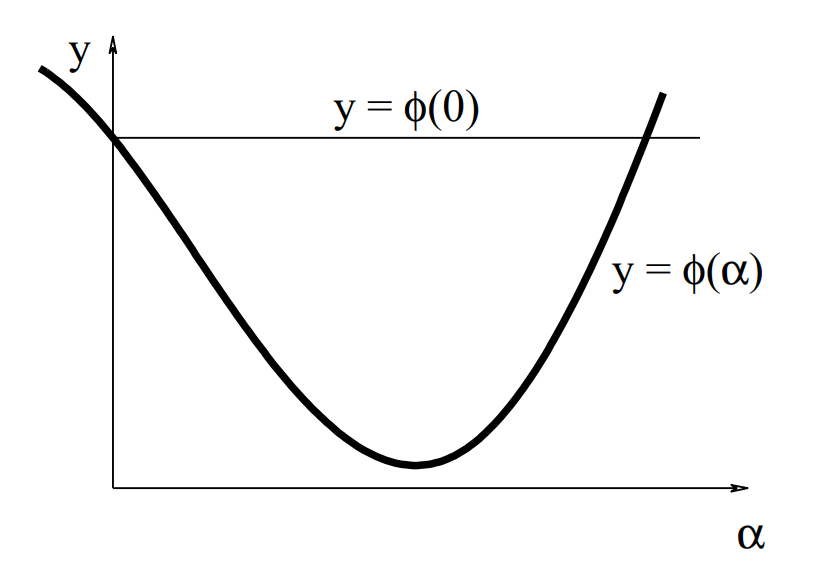
\includegraphics[width=3in]{line-search-cost-function.png}
        \caption{Loss value as a function $\varphi(\alpha)$ of the step length $\alpha$ when $\ve{h}$ is a descent direction \cite{Madsen:2004}.}
        \label{fig:line-search-cost-function}
    \end{figure}

    \item It is tempting to find $\alpha^* = \argmin_{\alpha > 0} \{ \varphi(\alpha) $. This results in an algorithm called {\bf exact line search}. However, this is still a hard optimization problem. Even if we allow ourselves to find a local minimizer instead of the global minimizer, literature still considers it not cost effective.
    
    \item Instead, what people do is {\bf inexact line search} where we produce an $\alpha$ value that is not too short and not too long.
    \begin{itemize}
        \item If $\alpha$ is too short, then $\varphi(0) - \varphi(\alpha)$ might be too small to call it an improvement, implying slow convergence.
        \item If $\alpha$ is too large, then $\varphi(\alpha)$ might be greater than $\varphi(0)$.
    \end{itemize}    
\end{itemize}

\subsubsection{Forms of Line Search Algorithm}

\begin{itemize}
    \item Inexact line search is generally an iterative algorithm.
    \begin{itemize}
        \item Starts with an initial guess $\alpha \gets \alpha^{(0)}$.
        \item Keeps updating the value of $\alpha$ until it satisfies some conditions.
    \end{itemize}

    \item In {\bf backtracking line search} \cite{Norcedal:2006} we start with a large initial guess, say $\alpha^{(0)} = 1$. We keep decreasing the value of $\alpha$ until it satisfies some condition. See Algorithm~\ref{algo:backtracking-line-search} for the pseudocode.
    
    \begin{algorithm}[t]
    \begin{algorithmic}
        \State $\alpha \gets \alpha^{(0)}$
        \While {$\alpha$ does not satisfy some conditions}
            \State Decrease $\alpha$.
        \EndWhile        
    \end{algorithmic}    
    \caption{Backtracking line search}
    \label{algo:backtracking-line-search}
    \end{algorithm}

    \item In {\bf interval binary search} \cite{Frandsen:2004}, we find an interval $[a,b]$ where an $\alpha$ value would be sampled from. After we sample $\alpha$, we would update $[a,b]$ like what we do in binary search: either turning it into $[a,\alpha]$ or $[\alpha,b]$. We keep doing this until our sampled $\alpha$ satisifed some conditions. The pseudocode of the algorithm is given in Algorithm~\ref{algo:interval-binary-search}.
        
    \begin{algorithm}[t]
    \begin{algorithmic}
        \State Find an interval $[a,b]$ where $\alpha$ should be sampled from.
        \State Sample $\alpha$ from $[a,b]$.
        \While {($\alpha$ does not satisfy some condition}                        
            \State Update $[a,b]$ to either $[a,\alpha]$ or $[\alpha,b]$.
            \State Sample $\alpha$ from $[a,b]$.
        \EndWhile        
        \State \Return $\alpha$
    \end{algorithmic}
    \caption{Interval binary search}
    \label{algo:interval-binary-search}
    \end{algorithm}
\end{itemize}

\subsubsection{Backtracking Armijo Line Search}

\begin{itemize}
    \item The first concrete example of a line search algorithm uses a condition called the ``Armijo condition''~\cite{Norcedal:2006} with the backtracking line search template.
    
    \item The {\bf Armijo condition} is as follow:
    \begin{align*}
        \varphi(\alpha) \leq \varphi(0) + c_1 \cdot \alpha \cdot \varphi'(0)
    \end{align*}
    where $0 < c_1 < 1$, and $c_1$ is often chosen to be around $10^{-4}$ \cite{Norcedal:2006}. It is depicted in Figure~\ref{fig:armijo-condition}.

    \begin{figure}
        \centering
        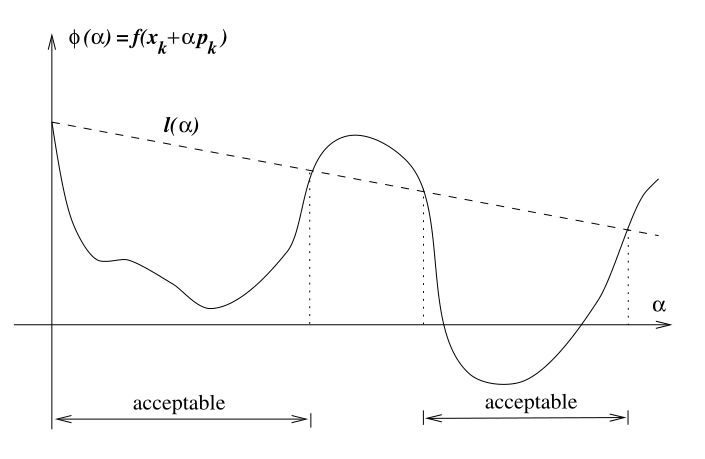
\includegraphics[width=4in]{armijo.png}
        \caption{The Armijo condition.}
        \label{fig:armijo-condition}        
    \end{figure}

    \item We note that the Armijo condition always hold at $\alpha = 0$.

    \item If we graph $\varphi$ as a function of $\alpha$, the Armijo condition requires that we find $\alpha$ such that $(\alpha, \varphi(\alpha))$ is below the line of slope $\gamma \varphi'(0)$ with vertical intercept $\varphi(0)$. In other words, it requires that the loss function decreases by some sufficient amount, determined by $\gamma$.
    \begin{itemize}
        \item As a result, the Armijo condition is sometimes referred to as the {\bf sufficient decrease condition}.        
    \end{itemize}

    \item The way we decrease $\alpha$ is to exponentially decay it. We pick a constant $0 < \rho < 1$ and update $\alpha \gets \rho \alpha$.

    \item The pseudocode of the full algorithm is given in Algorithm~\ref{algo:backtracking-armijo-line-search}. 
    
    \begin{algorithm}[t]
    \begin{algorithmic}
        \Procedure{Backtracking-Armijo-Line-Search}{}
        \State $\alpha \gets \alpha^{(0)}$
        \While {$\varphi(\alpha) > \varphi(0) + c_1 \alpha \varphi'(0)$}
            \State $\alpha \gets \rho \alpha$
        \EndWhile
        \State \Return $\alpha$
        \EndProcedure             
    \end{algorithmic}
    \caption{Backtracking Armijo line search}
    \label{algo:backtracking-armijo-line-search}
    \end{algorithm}

    \item The algorithm is gauranteed to terminate because the Armijo condition is always satisfied when $\alpha$ is low enough.
    
    \item A drawback of the algorithm is that there is no conditions that prevent $\alpha$ from being too small.
\end{itemize}

\subsubsection{Line Search with Wolfe Conditions}

\begin{itemize}    
    \item The {\bf Wolfe conditions} \cite{Norcedal:2006} consists of two conditions. The first condition ensures that $\alpha$ is small enough, and the second conditions ensures that $\alpha$ is not too small.
    \begin{itemize}
        \item The first condition is just the Armijo condition with the extra requirement that $c_2 < 0.5$ \cite{Madsen:2004}.
        \item The second condition is called the {\bf curvature condition}:
        \begin{align*}
            \varphi'(\alpha) \geq c_2 \cdot \varphi'(0)
        \end{align*}
        where $c_1 < c_2 < 1$, and $c_2$ is often picked to be much greater than $c_1$, typically in the order of $0.1$ \cite{Cao:2021}. See Figure~\ref{fig:wolfe-curvature-condition}. 
        
        \item The curvature condition requires that the gradient increases by some amount, making sure that the picked $\alpha$ yields $\ve{x}$ that is close to a stationary point.
    \end{itemize}    

    \begin{figure}
        \centering
        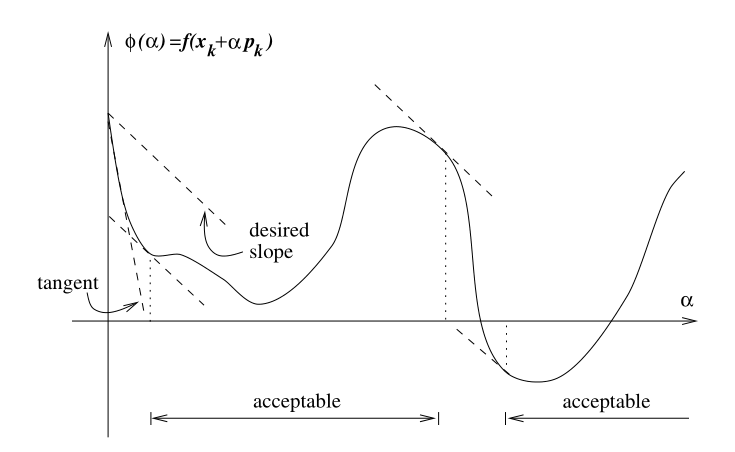
\includegraphics[width=4in]{wolfe-curvature-condition.png}
        \caption{Curvature condition \cite{Cao:2021,Norcedal:2006}.}
        \label{fig:wolfe-curvature-condition}
    \end{figure}

    \item There is a stronger version of the Wolfe conditions, and they are known as the {\bf strong Wolfe conditions}. The strong version differs from the regular one by changing the curvature condition to the following {\bf strong curvature condition}:
    \begin{align*}
        |\varphi'(\alpha)| \leq c_2 \cdot |\varphi'(0)|.
    \end{align*}
    In other words, while the curvature condition does not have limits on how positive $\varphi'(\alpha)$ can be, the strong curvature condition requires that $\varphi'(\alpha)$ cannot be too positive. It should be clear that the strong curvature condition implies the regular curvature condition.

    \item We note that \emph{both versions the curvature condition do not hold at $\alpha = 0$}.
    \begin{itemize}
        \item If we substitute $\alpha = 0$, the curvature condition reads $\varphi'(0) \geq \beta \cdot \varphi'(0)$. In other words, $(1 - \beta) \varphi'(0) \geq 0$. This is false because $1 - \beta > 0$, but $\varphi'(0) < 0$.
        \item On the other hand, the strong curvature condition reads $|\varphi'(0)| \leq c_2 \cdot |\varphi'(0)|$, which does not make sense because $|\varphi'(0)| > 0$ and $c_2 < 1$.
    \end{itemize}

    \item The following lemma shows that there always exist a step length that satisfy both versions of the Wolfe conditions given that the loss function $\mcal{L}$ is smooth and bounded below.
    
    \begin{lemma}
        Suppose that $\mcal{L}: \Real^n \ra \Real$ is continuously differentiable. Let $\ve{h}$ be a descent direction at $\ve{x}$. Assume that $\varphi(\alpha) = \mcal{L}(\ve{x} + \alpha \ve{h})$ is bounded below along ray $0 \leq \alpha < \infty$. Then, if $0 < c_1 < c_2 < 1$, there exists intervals of $\alpha$ values satisfying the Wolfe conditions and the strong Wolfe conditions.
    \end{lemma}

    The proof is in Norcedal and Wright \cite{Norcedal:2006}.
     
    \item The line search algorithm in this section also from Norcedal and Wright. Being a binary-search type algorithm, has two phases. We now discuss the first phase where an interval $[a,b]$ containing an $\alpha$ value that satisfies the \emph{strong} Wolfe condition is identified. The second phase is abstracted as a subroutine called $\Call{Zoom}{\cdot,\cdot}$. The implementation of this subroutine will be discussed later.
    \begin{itemize}
        \item The ``zoom'' name comes from Norcedal and Wright. I think this is not a good name.
    \end{itemize}

    \item The pseudocode of the first phase is given in Algorithm~\ref{algo:interval-binary-search-with-strong-wolfe-conditions}.
    
    \item The first phase uses the knowledge (stated but not proven in Norcedal and Wright that) that $[a,b]$ contains an $\alpha$ that satisflys the strong Wolfe conditions if at leaset one of the following three conditions hold:
    \begin{itemize}
        \item $b$ violates the Armijo condition. In other words, $\varphi(b) > \varphi(0) + c_1 b \varphi'(0)$.
        \item $\varphi(b) \geq \varphi(a)$.
        \item $\varphi'(b) \geq 0$.
    \end{itemize}
    
    \begin{algorithm}[t]
        \begin{algorithmic}
            \State $a \gets 0$
            \State $b \gets \min\{1, \alpha_{\max}\}$
            \While {{\bf true}}
                \If {$\varphi(b) > \varphi(0) + c_1 b \varphi'(0)$ {\bf or} $\varphi(b) \geq \varphi(a)$}
                    \State \Return $\Call{Zoom}{a,b}$
                \EndIf
                \If {$|\varphi'(b)| \leq c_2 |\varphi'(0)|$}
                    \State \Return $b$
                \EndIf                
                \If {$\varphi'(b) \geq 0$}
                    \State \Return $\Call{Zoom}{b,a}$
                \EndIf
                \State $a \gets b$
                \If {$a = \alpha_{\max}$}
                    \State \Return $\alpha_{\max}$
                \EndIf
                \State $b \gets \min\{ 2b, \alpha_{\max} \}$                
            \EndWhile            
        \end{algorithmic}
        \caption{Line search with strong Wolfe conditions}
        \label{algo:interval-binary-search-with-strong-wolfe-conditions}
    \end{algorithm}

    \item We now turn to the second phase, which is embodied by the $\Call{Zoom}{\cdot, \cdot}$ function. The pseudocode is given in Algorithm~\ref{algo:wolfe-zoom}.
    
    \begin{algorithm}[t]      
        \begin{algorithmic}
            \Procedure{Zoom}{$\alpha_{\mrm{lo}}, \alpha_{\mrm{hi}}$}
                \While {{\bf true}}
                    \State $\alpha \gets \Call{Get-Step-Length}{\alpha_{\mrm{lo}}, \alpha_{\mrm{hi}}}$
                    \If {$\varphi(\alpha) > \varphi(0) + c_1\alpha\varphi'(0)$ {\bf or} $\varphi(\alpha) \geq \varphi(\alpha_{\mrm{lo}})$}
                        \State $\alpha_{\mrm{hi}} \gets \alpha$
                        \State {\bf continue}
                    \EndIf
                    \If {$|\varphi(\alpha)| \leq c_2 |\varphi'(0)|$}
                        \State \Return $\alpha$
                    \EndIf
                    \If {$\varphi'(\alpha)(\alpha_{\mrm{hi}} - \alpha_{\mrm{lo}}) \geq 0$}
                        \State $\alpha_{\mrm{hi}} \gets \alpha_{\mrm{lo}}$
                    \EndIf
                    \State $\alpha_{\mrm{lo}} \gets \alpha$
                \EndWhile
            \EndProcedure
        \end{algorithmic}  
        \caption{The second phase of the line search with strong Wolfe conditions.}
        \label{algo:wolfe-zoom}
    \end{algorithm}

    \item The $\Call{Zoom}{\cdot,\cdot}$ function uses another function $\Call{Get-Step-Length}{\alpha_{\mrm{lo}},\alpha_{\mrm{hi}}}$ to sample an $\alpha$ from an interval bounded by $\alpha_{\mrm{lo}}$ and $\alpha_{\mrm{hi}}$. We shall discuss this function later.

    \item Let us discuss the parameters $\alpha_{\mrm{lo}}$ and $\alpha_{\mrm{hi}}$.
    \begin{itemize}
        \item We can see that $\Call{Zoom}{\cdot,\cdot}$ takes two arguments: $\alpha_{\mrm{lo}}$ and $\alpha_{\mrm{hi}}$.
        
        \item As should be appearent in the first phase (Algorithm~\ref{algo:interval-binary-search-with-strong-wolfe-conditions}), we do not require that $\alpha_{\mrm{lo}} < \alpha_{\mrm{hi}}$.
        
        \item Instead, we require that the following properties hold at all times.
        \begin{itemize}
            \item The interval bounded by $\alpha_{\mrm{lo}}$ and $\alpha_{\mrm{hi}}$ contains a step length that satisfy the strong Wolfe conditions.
            
            \item $\alpha_{\mrm{lo}}$ satisfies the Armijo condition. Moreover, among all $\alpha$ values that satisfied the Armijo condition that have been generated so far, $\varphi(\alpha_{\mrm{lo}})$ has the smallest value.
            
            \item $\alpha_{\mrm{hi}}$ is chosen so that $\varphi'(\alpha_{\mrm{lo}})(\alpha_{\mrm{hi}} - \alpha_{\mrm{lo}}) < 0$.
        \end{itemize}
    \end{itemize}
    
    \item One can check that the updates during the while loop of Algorithm~\ref{algo:wolfe-zoom} always maintain the above invariance. However, this might be quite tedious, and I will not be going through all the cases.
    
    \item Let us now discuss $\Call{Get-Step-Length}{\cdot,\cdot}$. Norcedal and Wright presents a sophisticated algorithm that requires approximating $\varphi$ with a cubic polynomial, but the presentation was not very clear to me. On the other hand, Frandsen \etal\ presents an algorithm based on approximating $\varphi$ with a cubic polynomial, and we shall present the algorithm in this note. The pseudocode is given in Algorithm~\ref{algo:zoom-get-step-length}.
    
    \begin{algorithm}[t]      
        \begin{algorithmic}
            \Procedure{Get-Step-Length}{$a, b$}
                \State $D \gets b - a$
                \State $c \gets (\varphi(b) - \varphi(a) - D \varphi'(a)) / D^2$
                \If {$c > 0$}
                    \State $\alpha \gets a - \varphi'(a) / (2c)$
                    \State $a \gets a + 0.1D$
                    \State $b \gets b - 0.1D$
                    \State $a,b \gets \min\{ a, b\}, \max\{a, b\}$
                    \State \Return $\min\{\max\{\alpha, a\}, b\}$.
                \Else
                    \State \Return $(a+b)/2$
                \EndIf
            \EndProcedure
        \end{algorithmic}  
        \caption{The second phase of the line search with strong Wolfe conditions.}
        \label{algo:zoom-get-step-length}
    \end{algorithm}

    \item To explain how the function works, first note that the polynomial
    \begin{align*}
        \psi(\alpha) = \varphi(a) + \varphi'(a)(\alpha-a) + c(\alpha-a)^2,
    \end{align*}
    where
    \begin{align*}
        c = \frac{\varphi(b) - \varphi(a) - \varphi'(a)(b-a)}{(b-a)^2},
    \end{align*}
    satisfies the following properties:
    \begin{itemize}
        \item $\psi(a) = \varphi(a)$,
        \item $\psi'(a) = \varphi'(a)$, and
        \item $\psi(b) = \varphi(b)$.
    \end{itemize}
    So, $\psi(t)$ is an approximation of $\varphi(\alpha)$ in the interval bounded by $a$ and $b$.

    \item If $c > 0$, then the polynomial is a parabola that opens up, so it has a global minimum. The minimizer $\alpha$ is determined by
    \begin{align*}
        \psi'(\alpha) &= 0 \\
        \varphi'(a) + 2c(\alpha - a) &= 0  \\
        \alpha &= a - \frac{\varphi'(a)}{2c}.
    \end{align*}
    As a result, we choose this value as the candicate. However, $\alpha$ might fall outside the interval bounded by $a$ and $b$ or too close to $a$ and $b$ to prevent meaningful interval shrinking. So, we bound $\alpha$ so that the interval shrinks by at least $10\%$.

    \item If $c \leq 0$, then the polynomial does not have a global minimum, and the minimum is at one of the endpoints. In this case, we just chooise $\alpha$ to be the middle point between $a$ and $b$.
    
    \item One thing to be aware of is that line search can be expensive because one needs to evaluate $\varphi(\alpha)$ and $\varphi'(\alpha)$ many times. When implementing one of these algorithms, we need to be vigilant and now overcompute stuffs.
\end{itemize}

\subsection{Trust Region and Damped Methods} \label{sec:trust-region-and-damped-methods}

\begin{itemize}    
    \item We assume that we have a function $\mathtt{L}: \Real^n \ra \Real$ that models the behavior of $\mcal{L}$ in the neighborhood of the current solution $\ve{x}$.
    \begin{align*}
        \mcal{L}(x + \ve{h}) \approx \mathtt{L}(\ve{h}).
    \end{align*}
    
    \item Usually, the model $\mathtt{L}$ is a quadratic function of the form:
    \begin{align*}
        \mathtt{L}(\ve{h}) = c + \ve{b}^T \ve{h} + \frac{1}{2} \ve{h}^T A \ve{h}.
    \end{align*}
    where $c \in \Real$, $\ve{b} \in \Real^n$, and $A \in \Real^{n \times n}$ is a symmetric matrix.

    \item In general, we want $\mathtt{L}$ to with $\mcal{L}$ up to first order. As a result, we typically choose $c = \mcal{L}(\ve{x})$ and $\ve{b} = \nabla\mcal{L}(\ve{x})^T$. The matrix $A$ is either the Hessian of $\mcal{L}$ at $\ve{x}$ or some approximation of it.
    
    \item In a {\bf trust region method}, we assume that we know a positive constant $\Delta$ such that the model is sufficiently accurate inside a ball with radius $\Delta$ around $\ve{x}$. Then, we choose the update direction by computing
    \begin{align}
        \ve{h} = \argmin_{\| \ve{h} \| \leq \Delta} \{ \mathtt{L}(\ve{h}) \}. \label{eq:trust-region-method-optimization}
    \end{align}

    \item In a {\bf damped method}, we use the following minimization problem instead:
    \begin{align}
        \ve{h} = \argmin_{\ve{h}} \bigg\{ \mathtt{L}(\ve{h}) + \frac{1}{2}\mu \ve{h}^T \ve{h} \bigg\}. \label{eq:damped-method-optimization}
    \end{align}
    The term $\frac{1}{2}\mu\ve{h}^T \ve{h}$ penalize large update direction.

    \item The template for a trust region and damped method is given in Algorithm~\ref{algo:trust-region-method}.    

    \begin{algorithm}
        \begin{algorithmic}
            \While {not satisifed}
                \State Compute $\ve{h}$ according to \eqref{eq:trust-region-method-optimization} or \eqref{eq:damped-method-optimization}.
                \If {$\mcal{L}(x + \ve{h}) < \mcal{L}(\ve{x})$}
                    \State $\ve{x} \gets \ve{x} + \ve{h}$
                \EndIf
                \State Update $\mathtt{L}$ and $\Delta$ or $\mu$.
            \EndWhile
        \end{algorithmic}
        \caption{A template for trusted region and damped methods.}
        \label{algo:trust-region-method}
    \end{algorithm}

    \item We see that the trust region method is quite different from line search.
    \begin{itemize}
        \item In line search, we come up with an update direction first. Then, we choose a step length to update along that direction.
        \item In trust region method, we start with an initial guess of $\Delta$ and $\mathtt{L}$. We find an update direction $\ve{h}$. If $\ve{h}$ results in an improvement, we update along $\ve{h}$ with step length $\alpha = 1$. Otherwise, we do not move (i.e., $\alpha = 0)$. In any case, we need to update $\Delta$ and $\mathtt{L}$.
        \begin{itemize}
            \item If the previous update fails, we generally shrink $\Delta$ to make the model more accurate.
            \item If the previous update success, we need to update $\mathcal{L}$ to take into account the new value of $\ve{x}$. We may then set $\Delta$ to a high value to make sure that we catch potential large updates at a new point.
        \end{itemize}
    \end{itemize}    

    \item The improvement of the update step is determined by the {\bf gain ratio} \cite{Madsen:2004}:
    \begin{align*}
        \varrho = \frac{\mcal{L}(\ve{x}) - \mcal{L}(\ve{x}+\ve{h})}{\mathtt{L}(\ve{0}) - \mathtt{L}(\ve{h})}.
    \end{align*}
    The nominator is called the {\bf actual decrease}, and the denominator is called the {\bf predicted decrease} \cite{Norcedal:2006}. By construction, the predicted decrease is always positive.

    \item With a trust region method, the following strategy for updating $\Delta$ is widely used.
    \medskip
    \begin{algorithmic}
        \If {$\varrho < 0.25$}
            \State $\Delta \gets \Delta / 2$
        \Else
            \State $\Delta \gets \max\{ \Delta, 3 \| \ve{h} \| \}$
        \EndIf
    \end{algorithmic}

    \item In a damped method, a small $\varrho$ indicates that we should increase the damping factor $\mu$. Otherwise, damping might be decreased because the model is a good approximation. A widely used strategy is proposed by Marquardt for the famed Levenberg--Marquardt algorithm \cite{Marquadrt:1963}.
    \medskip
    \begin{algorithmic}
        \If {$\varrho < 0.25$}
            \State $\mu \gets 2 \mu$        
        \EndIf
        \If {$\varrho > 0.75$}
            \State $\mu \gets \mu / 3$
        \EndIf
    \end{algorithmic}

    \item The method above is not sensitive to minor changes in the thresholds $0.25$ and $0.75$ or the numbers $p_1 = 2$ and $p_2 = 3$. However, $p_1$ and $p_2$ should be chosen so that the $\mu$ values would not oscillate, which would slow down convergence.
    
    \pagebreak
    
    \item It turns out that the threshold $0.25$ and $0.75$ are not that good. The following strategy by Nielsen performs better \cite{Nielsen:1999}.
    \begin{algorithmic}
        \State $\nu \gets 2$
        \If {$\varrho > 0$}
            \State $\mu \gets \mu \max\{ 1/3, 1 - (2\varrho-1)^3\}$
            \State $\nu \gets 2$
        \Else
            \State $\mu \gets \mu \nu$
            \State $\nu \gets 2\nu$
        \EndIf
    \end{algorithmic}

    \item In a damped method, the update $\ve{h}$ is computed by finding a statinary point of the function
    \begin{align*}
        \psi_\mu(\ve{h}) 
        &= \mcal{L}(\ve{h}) + \frac{1}{2}\mu\ve{h}^T\ve{h} \\
        &= c + \ve{b}^T \ve{h} + \frac{1}{2} \ve{h}^T A \ve{h} + \frac{1}{2}\mu \ve{h}^T \ve{h} \\
        &= c + \ve{b}^T \ve{h} + \frac{1}{2} \ve{h}^T (A + \mu I) \ve{h}.
    \end{align*}
    This requires that
    \begin{align*}
        (\nabla \psi_\mu(\ve{h}))^T = \ve{0},        
    \end{align*}
    or
    \begin{align*}
        (A + \mu I)\ve{h} + \ve{b} &= 0 \\
        \ve{h} &= -(A + \mu I)^{-1} \ve{b}.
    \end{align*}
    If $\mu$ is sufficiently large, the symmetric matrix $A + \mu I$ is positive definite, and $\ve{h}$ would be a minimizer of $\psi_u$.

    \item In a trust region method, the step $\ve{h}$ is the solution to the \emph{constrained} optimization problem
    \begin{itemize}
        \item[] minimize $\mathcal{L}(\ve{h})$
        \item[] subject to $\ve{h}^T\ve{h} \leq \Delta^2$
    \end{itemize}
    However, we will not discuss how to solve this problem in this note.
\end{itemize}

\subsection{Damped Newton's Method}

\begin{itemize}
    \item An illuminating example of damped methods is the {\bf damped Newton's method}.
    
    \item The model $\mathtt{L}(\ve{h})$ is given by
    \begin{align*}
        \mathtt{L}(\ve{h}) = \mcal{L}(\ve{x}) + \nabla \mcal{L}(\ve{x})\ve{h} + \frac{1}{2} \ve{h}^T H_{\mcal{L}}(\ve{x}) \ve{h}.
    \end{align*}

    \item The update direction $\ve{h}_{\mrm{dn}}$ takes the form
    \begin{align*}
        (H_{\mcal{L}}(\ve{x}) + \mu I) \ve{h}_{\mrm{dn}} = - \nabla \mcal{L}(\ve{x})^T.
    \end{align*}

    \item When $\mu$ is small, the equation above becomes close to the equation of Newont's method, and the method's behavior becomes similar to that of Newton's method.
    
    \item However, when $\mu$ is large, we have that $\ve{h}_{\mrm{dm}} \approx -\frac{1}{\mu} \mcal{L}(\ve{x})^T$, which is a short step in the direction of the gradient.
    
    \item As a result, we can think of the damped Newton's method has a hybrid between gradient descent and Newton's method.
\end{itemize}

\section{Non-Linear Least Squares}

\begin{itemize}
    \item We are given a vector function $\ve{f}: \Real^n \ra \Real^m$, and we want to find
    \begin{align*}
        \ve{x}^* = \argmin_{\ve{x}} \bigg\{ \frac{1}{2} \| \ve{f}(\ve{x}) \|^2 \bigg\} = \argmin_{\ve{x}} \bigg\{ \frac{1}{2} \ve{f}(\ve{x})^T \ve{f}(\ve{x}) \bigg\} 
    \end{align*}

    \item Provided that $\ve{f}$ has continuous second partial derivatives, we have that
    \begin{align*}
        \ve{f}(\ve{x} + \ve{h}) = \ve{f}(\ve{x}) + \nabla \ve{f}(\ve{x}) \ve{h} + O(\| \ve{h}\|^2)
    \end{align*}
    where $\nabla \ve{f}(\ve{x}) \in \Real^{m \times n}$ is the derivative of $\ve{f}$ at $\ve{x}$. This is often called the {\bf Jacobian matrix} and is usually abbreviate as just $J(\ve{x})$.

    \item Our loss function is given by
    \begin{align*}
        \mcal{L}(\ve{x}) = \frac{1}{2} \ve{f}(\ve{x})^T \ve{f}(\ve{x}).
    \end{align*}
    The gradient of the loss function is given by
    \begin{align*}
        \nabla \mcal{L}(\ve{x}) = \ve{f}(\ve{x})^T J(\ve{x}).
    \end{align*}
    Moreover, the Hessian is given by
    \begin{align*}
        H_{\mcal{L}}(\ve{x}) = J(\ve{x})^T J(\ve{x}) + \sum_{i=1}^m f_i(\ve{x}) H_{f_i}(\ve{x}).
    \end{align*}
\end{itemize}

\subsection{The Gauss--Newton Method}

\begin{itemize}
    \item The method is based on a linear approximation to the components of $\ve{f}$. When $\| \ve{h} \|$ is small, we have that
    \begin{align*}
        \ve{f}(\ve{x} + \ve{h}) \approx \ves{\ell}(\ve{h}) = \ve{f}(\ve{x}) + J(\ve{x})\ve{h}.
    \end{align*}
    As a result,
    \begin{align*}
        \mcal{L}(\ve{x}+\ve{h})         
        &= \frac{1}{2} \ve{f}(\ve{x})^T \ve{f}(\ve{x}) \\
        &\approx \frac{1}{2} \ves{\ell}(\ve{x})^T \ves{\ell}(\ve{x}) \\
        &= \frac{1}{2} (\ve{f}(\ve{x}) + J(\ve{x})\ve{h})^T (\ve{f}(\ve{x}) + J(\ve{x})\ve{h}) \\
        &= \frac{1}{2} \ve{f}(\ve{x})^T \ve{f}(\ve{x}) + \ve{h}^T J(\ve{x})^T \ve{f}(\ve{x}) + \frac{1}{2} \ve{h}^T J(\ve{x})^T J(\ve{x}) \ve{h} \\
        &= \mcal{L}(\ve{x}) + \ve{h}^T J(\ve{x})^T \ve{f}(\ve{x}) + \frac{1}{2} \ve{h}^T J(\ve{x})^T J(\ve{x}) \ve{h} 
    \end{align*}

    \item Let
    \begin{align*}
        \mathtt{L}(\ve{h}) = \mcal{L}(\ve{x}) + \ve{h}^T J(\ve{x})^T \ve{f}(\ve{x}) + \frac{1}{2} \ve{h}^T J(\ve{x})^T J(\ve{x}) \ve{h}.
    \end{align*}
    The Gauss--Newton update $\ve{h}_{\mrm{gn}}$ minimizes $\mathtt{L}(\ve{h})$:
    \begin{align*}
        \ve{h}_{\mrm{gn}} = \argmin_{\ve{h}} \big\{ \mathtt{L}(\ve{h}) \big\}
    \end{align*}

    \item We have that
    \begin{itemize}
        \item $\nabla \mathtt{L}(\ve{h}) = \ve{f}(\ve{x})^T J(\ve{x})  + \ve{h}^T J(\ve{x})^TJ(\ve{x})$.
        \item $H_{\mathtt{L}}(\ve{h}) = J(\ve{x})^T J(\ve{x})$.
    \end{itemize}

    \item To find $\ve{h}_{\mrm{gn}}$, we set $(\nabla \mathtt{L}(\ve{h}))^T$ to $\ve{0}$, which gives
    \begin{align*}
        J(\ve{x})^T \ve{f}(\ve{x}) + J(\ve{x})^TJ(\ve{x})\ve{h} &= \ve{0} \\
        \ve{h} &= - \big(J(\ve{x})^TJ(\ve{x})\big)^{-1} J(\ve{x})^T \ve{f}(\ve{x}),
    \end{align*}
     If $\ve{J}(\ve{x})$ has full rank, we have that $J(\ve{x})^TJ(\ve{x})$ would be positive definite, and $\ve{h}_{\mrm{gn}}$ would be the unique minimizer of $\mathtt{L}(\ve{h})$.

    \item A typical implementation of the Gauss--Newton method is given in Algorithm~\ref{algo:gauss-newton}.

    \begin{algorithm}[t]
        \begin{algorithmic}
            \State Compute $\ve{h}_{\mrm{gn}} =  - \big(J(\ve{x})^TJ(\ve{x})\big)^{-1} J(\ve{x})^T \ve{f}(\ve{x})$.
            \State Find step length $\alpha$ with a line search.
            \State $\ve{x} \gets \ve{x} + \alpha \ve{h}_{\mrm{gn}}$
        \end{algorithmic}
        \caption{Gauss--Newton update step.}
        \label{algo:gauss-newton}
    \end{algorithm}

    \item The method with line search has gauranteed convergence provided that $\{ \ve{x} : \mcal{L}(\ve{x}) \leq \mcal{L}(\ve{x}^{(0)}) \}$ is bounded, and the Jacobian $J(\ve{x})$ has full rank in all steps.
    
    \item While Newton's method have quadratic convergence, the convergence of Gauss--Newton method is generally linear.
    \begin{itemize}
        \item The surprising thing is that the loss value at the local minimizer $\mcal{L}(\ve{x}^*)$ actually controls the convergence speed. See Madset \etal~\cite{Madsen:2004}.
    \end{itemize}    
\end{itemize}

\subsection{The Levenberg--Marquardt Method}

\begin{itemize}
    \item Levenberg \cite{Levenberg:1944} and later Marquardt \cite{Marquadrt:1963} suggests the use of a damped Gauss--Newton method.
    
    \item The update direction $\ve{h}_{\mrm{lm}}$ is determined by solving the following equation:
    \begin{align*}
        (J(\ve{x})^TJ(\ve{x}) + \mu I) \ve{h}_{\mrm{lm}} = - J(\ve{x})^T \ve{f}(\ve{x}).
    \end{align*}

    \item The damping parameter $\mu$ has several effects.
    \begin{itemize}
        \item For $\mu > 0$, the matrix on the LHS is positive definite. This ensures that $\ve{h}_{\mrm{lm}}$ is a descent direction of the model $\mathtt{L}$.
        
        \item For large values of $\mu$, we get that $\ve{h}_{\mrm{lm}} \approx - J(\ve{x})^T \ve{f}(\ve{x}) / \mu = - \nabla{L}(\ve{x})/\mu$, which is a short step in the direction of the gradient of the loss function. This is good if $\ve{x}$ is far from the solution.
        
        \item If $\mu$ is very small, then $\ve{h}_{\mrm{lm}} \approx \ve{h}_{\mrm{gn}}$, which is a good step in the final stages of the iterations. If $\mcal{L}(\ve{x}^*) = 0$, we  can get quadratic final convergence.
    \end{itemize}

    \item As a damped method, we do not need line search to determine the step length. However, we must come up with a way to update $\mu$.
    
    \item The initial value of $\mu$ should be related to the size of the elements in $A^{(0)} = J(\ve{x}^{(0)})^T J(\ve{x}^{(0)})$. It is typically set to
    \begin{align*}
        \mu^{(0)} = \tau \cdot \max_{1 \leq i \leq n} \{ a^{(0)}_{ii} \} 
    \end{align*}
    where $\tau$ is a constant specified by the user.
    \begin{itemize}
        \item The algorithm is not very sensitive to the choice of $\tau$.
        \item As a rule of thumb, one should use a small value. For example, $\tau = 10^{-6}$ if $\ve{x}^{(0)}$ is believed to be a good appriximation of $\ve{x}^*$.
        \item Otherise, we use $\tau = 10^{-3}$ or $\tau = 1$.
    \end{itemize}

    \item Updating $\mu$ is controlled by the gain ratio
    \begin{align*}
        \varrho = \frac{\mathcal{L}(\ve{x}) - \mathcal{L}(\ve{x} + \ve{h}_{\mrm{lm}})}{\mathtt{L}(\ve{0}) - \mathtt{L}(\ve{h}_{\mrm{lm}})}.
    \end{align*}
    The denominator is given by
    \begin{align*}
        \mathtt{L}(\ve{0}) - \mathtt{L}(\ve{h}_{\mrm{lm}})
        &= -\ve{h_{\mrm{lm}}}^T J(\ve{x})^T \ve{f}(\ve{x}) - \frac{1}{2} \ve{h}_{\mrm{lm}}^T J(\ve{x})^T J(\ve{x}) \ve{h}_{\mrm{lm}} \\
        &= \ve{h_{\mrm{lm}}}^T (J(\ve{x})^TJ(\ve{x}) + \mu I) \ve{h}_{\mrm{lm}}  - \frac{1}{2} \ve{h}_{\mrm{lm}}^T J(\ve{x})^T J(\ve{x}) \ve{h}_{\mrm{lm}} \\
        &= \frac{1}{2} \ve{h_{\mrm{lm}}}^T (2J(\ve{x})^TJ(\ve{x}) + 2\mu I) \ve{h}_{\mrm{lm}}  - \frac{1}{2} \ve{h}_{\mrm{lm}}^T J(\ve{x})^T J(\ve{x}) \ve{h}_{\mrm{lm}} \\
        &= \frac{1}{2} \ve{h_{\mrm{lm}}}^T (J(\ve{x})^TJ(\ve{x}) + 2\mu I) \ve{h}_{\mrm{lm}} \\
        &= \frac{1}{2} \ve{h_{\mrm{lm}}}^T \big(( J(\ve{x})^TJ(\ve{x}) + \mu I)  + \mu I\big) \ve{h}_{\mrm{lm}} \\
        &= \frac{1}{2} \ve{h_{\mrm{lm}}}^T \big(\mu \ve{h}_{\mrm{lm}} - J(\ve{x})^T \ve{f}(\ve{x})).
    \end{align*}
    Because $\ve{h}_{\mrm{lm}}$ is a descent direction, it must be that $- \ve{h}_{\mrm{lm}}J(\ve{x})^T \ve{f}(\ve{x})$ must be positive. As a result, the denominator is always positive.

    \item To update $\mu$, we can use Nielsen's rule \cite{Nielsen:1999} in Section~\ref{sec:trust-region-and-damped-methods}.
    
    \item Now, we need to decide when the stop the algorithm. There are three criteria.
    \begin{itemize}
        \item First, we should stop when we reach a stationary point. This means that $(\nabla \mcal{L}(\ve{x}))^T = J(\ve{x})^T \ve{f}(x) = \ve{0}$. As a result, we can use
        \begin{align*}
            \| J(\ve{x})^T \ve{f}(x) \|_{\infty} \leq \varepsilon_1
        \end{align*}
        where $\varepsilon_1$ is a small positive constant chosen by the user.

        \item Another criteria is to stop when the change in $\ve{x}$ is small.
        \begin{align*}
            \| \ve{x}_{\mrm{new}} - \ve{x} \| \leq \varepsilon_2 (\| \ve{x}\| + \varepsilon_2)
        \end{align*}
        where $\varepsilon_2$ is another small positive constant chosen by the user. This expression gives a gradual change from relative size $\varepsilon_2 \| \ve{x}\|$ when $\| \ve{x}\|$ is large and to absolute size $\varepsilon_2^2$ when $\| \ve{x} \|$ is close to $\ve{0}$.

        \item Lastly, the algorithm should terminate when a maximum number of iterations, chosen by the user, is reached.
    \end{itemize}

    \item The pseudocode of the Levenberg--Marquardt algorithm is given in Algorithm~\ref{algo:levenberg-marquardt}.

    \begin{algorithm}[t]
        \begin{algorithmic}
            \State $k \gets 0$
            \State $\nu \gets 2$
            \State $\ve{x} \gets \ve{x}^{(0)}$
            \State $A = J(\ve{x})^T J(\ve{x})$
            \State $\ve{g} \gets J(\ve{x})^T \ve{f}(\ve{x})$
            \State $\mu = \tau \cdot \max_{1 \leq i \leq n} \{a_{ii}\}$
            \While {$\| \ve{g} \|_\infty > \varepsilon_1$ {\bf and} $k \leq k_{\max}$}
                \State Determine $\ve{h}_{\mrm{lm}}$ by solving $(A + \mu I)\ve{h}_{\mrm{lm}} = \ve{g}$.
                \If {$\| \ve{h}_{\mrm{lm}} \leq \varepsilon_2 (\| \ve{x}\| + \varepsilon_2)$}
                    \State \Return $\ve{x}$
                \EndIf
                \State $\ve{x}_{\mrm{new}} \gets \ve{x} + \ve{h}_{\mrm{lm}}$
                \State $\varrho \gets (\mcal{L}(\ve{x}) - \mcal{L}(\ve{x}_{\mrm{new}})) / (\mathtt{L}(\ve{0}) - \mathtt{L}(\ve{h}_{\mrm{lm}}))$
                \If {$\varrho > 0$}
                    \State $\ve{x} \gets \ve{x}_{\mrm{new}}$
                    \State $A = J(\ve{x})^T J(\ve{x})$
                    \State $\ve{g} \gets J(\ve{x})^T \ve{f}(\ve{x})$
                    \State $\mu \gets \mu \cdot \max\{ \frac{1}{3}, 1 - (2\varrho -1)^3 \}$
                    \State $\nu \gets 2$
                \Else
                    \State $\mu \gets \mu \nu$
                    \State $\nu \gets 2\nu$
                \EndIf
                \State $k \gets k+1$
            \EndWhile
            \State \Return $\ve{x}$
        \end{algorithmic}
        \caption{The Levenberg--Marquardt algorithm.}
        \label{algo:levenberg-marquardt}
    \end{algorithm}
\end{itemize}


\bibliographystyle{acm}
\bibliography{nonlinear-least-square-algo}
\end{document}